%%%%%%%%%%%%%%%%%%%%%%%%%%%%%%%%%%%%%%%%%
% Short Sectioned Assignment
% LaTeX Template
% Version 1.0 (5/5/12)
%
% This template has been downloaded from:
% http://www.LaTeXTemplates.com
%
% Original author:
% Frits Wenneker (http://www.howtotex.com)
%
% License:
% CC BY-NC-SA 3.0 (http://creativecommons.org/licenses/by-nc-sa/3.0/)
%
%%%%%%%%%%%%%%%%%%%%%%%%%%%%%%%%%%%%%%%%%

%----------------------------------------------------------------------------------------
%	PACKAGES AND OTHER DOCUMENT CONFIGURATIONS
%----------------------------------------------------------------------------------------

\documentclass[paper=a4, fontsize=11pt]{scrartcl} % A4 paper and 11pt font size

\usepackage[T1]{fontenc} % Use 8-bit encoding that has 256 glyphs
\usepackage{fourier} % Use the Adobe Utopia font for the document - comment this line to return to the LaTeX default
\usepackage[english]{babel} % English language/hyphenation
\usepackage{amsmath,amsfonts,amsthm} % Math packages
\usepackage[utf8]{inputenc}

\usepackage{graphicx}

\usepackage{lipsum} % Used for inserting dummy 'Lorem ipsum' text into the template

\usepackage{sectsty} % Allows customizing section commands
\allsectionsfont{\centering \normalfont\scshape} % Make all sections centered, the default font and small caps

\usepackage{fancyhdr} % Custom headers and footers
\pagestyle{fancyplain} % Makes all pages in the document conform to the custom headers and footers
\fancyhead{} % No page header - if you want one, create it in the same way as the footers below
\fancyfoot[L]{} % Empty left footer
\fancyfoot[C]{} % Empty center footer
\fancyfoot[R]{\thepage} % Page numbering for right footer
\renewcommand{\headrulewidth}{0pt} % Remove header underlines
\renewcommand{\footrulewidth}{0pt} % Remove footer underlines
\setlength{\headheight}{13.6pt} % Customize the height of the header

\numberwithin{equation}{section} % Number equations within sections (i.e. 1.1, 1.2, 2.1, 2.2 instead of 1, 2, 3, 4)
\numberwithin{figure}{section} % Number figures within sections (i.e. 1.1, 1.2, 2.1, 2.2 instead of 1, 2, 3, 4)
\numberwithin{table}{section} % Number tables within sections (i.e. 1.1, 1.2, 2.1, 2.2 instead of 1, 2, 3, 4)

\setlength\parindent{0pt} % Removes all indentation from paragraphs - comment this line for an assignment with lots of text

%----------------------------------------------------------------------------------------
%	TITLE SECTION
%----------------------------------------------------------------------------------------

\newcommand{\horrule}[1]{\rule{\linewidth}{#1}} % Create horizontal rule command with 1 argument of height

\title{	
\normalfont \normalsize 
\textsc{TDT4200 - Parallell Computing, IDI, NTNU} \\ [25pt] % Your university, school and/or department name(s)
\horrule{0.5pt} \\[0.4cm] % Thin top horizontal rule
\huge Problem set 1 - Theory \\ % The assignment title
\horrule{2pt} \\[0.5cm] % Thick bottom horizontal rule
}

\author{Øyvind Robertsen} % Your name

\date{\normalsize\today} % Today's date or a custom date

\begin{document}

\maketitle % Print the title

%----------------------------------------------------------------------------------------
%	PROBLEM 1
%----------------------------------------------------------------------------------------

\section{General Theory}

\subsection{Flynn's Taxonomy}


\begin{table}[h!]
    \begin{tabular}{|p{0.2\linewidth}|p{0.33\linewidth}|p{0.33\linewidth}|}
        \hline
    ~             & Single Instruction                                                                                  & Multiple Instruction                                                                   \\ \hline
        Single Data   & A single processing unit performing one instruction at a time on a single data element. (SISD)             & Multiple processing units performing different instructions on the same data element. (MISD)  \\ \hline
        Multiple Data & Multiple processing units performing the same instructions on different data elements in parallell. (SIMD) & Multiple processing units performing different instructions on different data elements. (MIMD) \\ \hline
    \end{tabular}
\end{table}

Additionaly, MIMD is often subcategorized into SPMD (Single Program, Multiple Data) and MPMD (Multiple program, Multiple Data).
SPMD refers to executing the same program across several processes, each operating on different datasets.
MPMD, on the other hand, executes at least two different programs, often in a host/node or manager/worker configuration.

MPI falls under SPMD in this categorization. We instantiate several processes of the same program, where each process itself decides its behavior based on its rank.

\subsection{Shared Memory}

On shared memory systems, all cores share access to the computers memory.
MPI processes running on such a system defaults to using shared memory to facilitate message passing between processes.

\subsection{Distributed Memory}

On distributed memory systems, each core has its own, private memory.
MPI processes running on these systems uses network interfaces to facilitate message passing between processes.

\section{Code Theory}

\subsection{Communicational bottlenecks}

My implementation suffers from a communicational bottleneck in process 0, which is responsible for gathering the results from each of the other processes.
Since the computation we want to perform on each of the results of the other processes is a fast one, namely adding, and there will be low variance in the time necessary to produce the result from the non-rank-0 processes, we will not be greatly effected by this bottleneck for this specific program.

One way of reducing the impact of this bottleneck would be to not block the rank-0 process while it waits for the result from each other process, but rather to sum results from the worker-processes as they become available in a non-blocking fashion.
There are non-blocking \texttt{Send/Recv}-implementations that can be used.

Alternatively, we could distribute the collection of results in a treelike structure of processes. (Rank 0 receives and sums results from two processes that have themselves summed the results of two subprocesses, and so on.)


\subsection{Computational bottlenecks}


Computing $\log{n}$ is the most expensive single operation my implementation performs.
It also performs this operation n times regardless of how much we parallellize the solution.
We can however improve on this brute force application by approximating the value of the sum with an integral.

\begin{gather*}
    \sum_{i}^{n} \frac{1}{\log{n}} = \int_{i}^{n} \frac{1}{\log{x}} dx
\end{gather*}

We can approximate this using, for instance, the trapezoidal rule.



\section{Code analysis}

\subsection{Total operations}

The total number of operations my program performs is $O(n)$.
The number of operations per process is $O(\frac{n}{P})$

\subsection{Total MPI operations}

The total amount of MPI operations in my program is $O(P)$.

\subsection{Average MPI operations}

The average amount of MPI operations per process is $O(1)$.

\subsection{Maximum MPI operations}

The maximum amount of MPI operations performed by any process is the number of MPI-operations performed by the "master"-process, $P_0$.
This process performs $O(P)$ MPI operations.

\subsection{Run-time differences}

The data was gathered by running my parallel implementation on \texttt{ITS-015-12} with all the different input variations.

\begin{figure}[H]
    \centering
    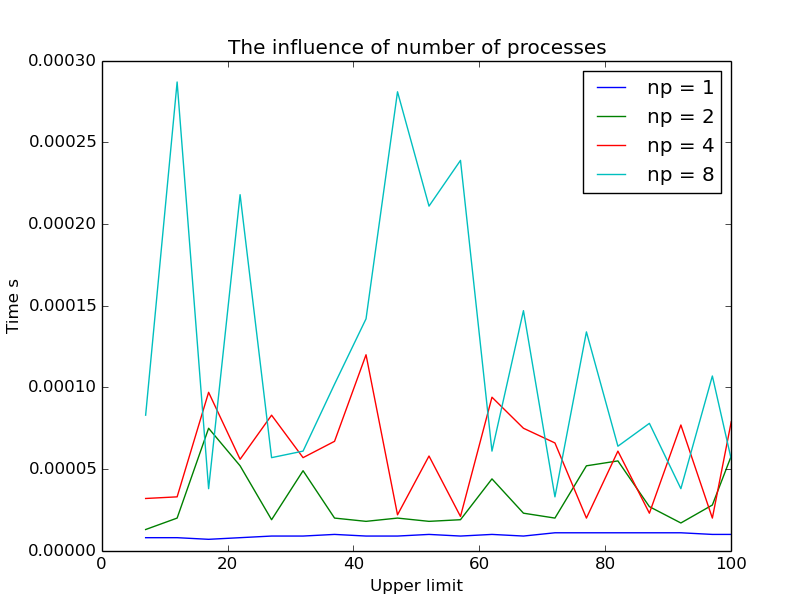
\includegraphics[width=\linewidth]{low.png}
    \caption{Run-time for evenly incrementing ranges within $2 \rightarrow 100$} \label{fig:low}
\end{figure}

\begin{figure}[H]
    \centering
    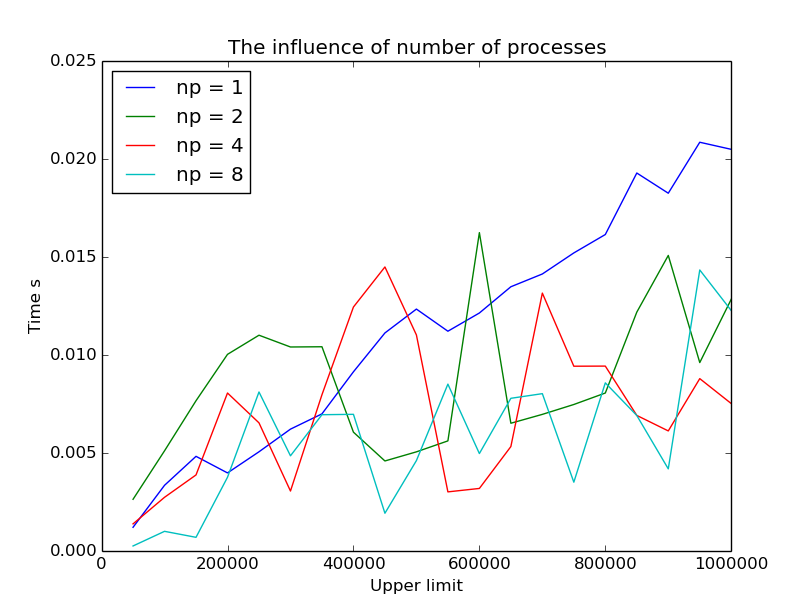
\includegraphics[width=\linewidth]{med.png}
    \caption{Run-time for evenly incrementing ranges within $2 \rightarrow 1000000$} \label{fig:med}
\end{figure}

\begin{figure}[H]
    \centering
    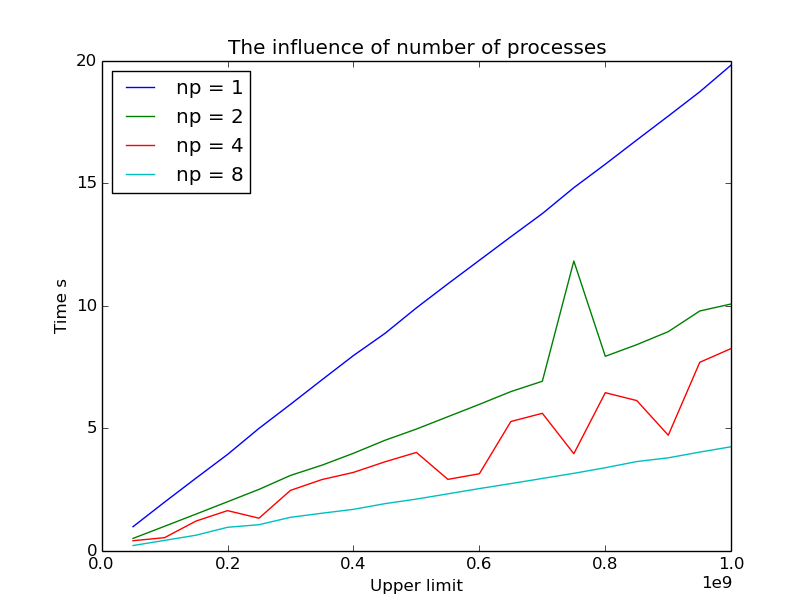
\includegraphics[width=\linewidth]{high.png}
    \caption{Run-time for evenly incrementing ranges within $2 \rightarrow 1000000000$} \label{fig:high}
\end{figure}

%----------------------------------------------------------------------------------------

\end{document}

